\section{Agent-Coordinated Task-Level Operation}
\label{sec:closed-loop-operation}

\begin{figure*}[!t]
\centering
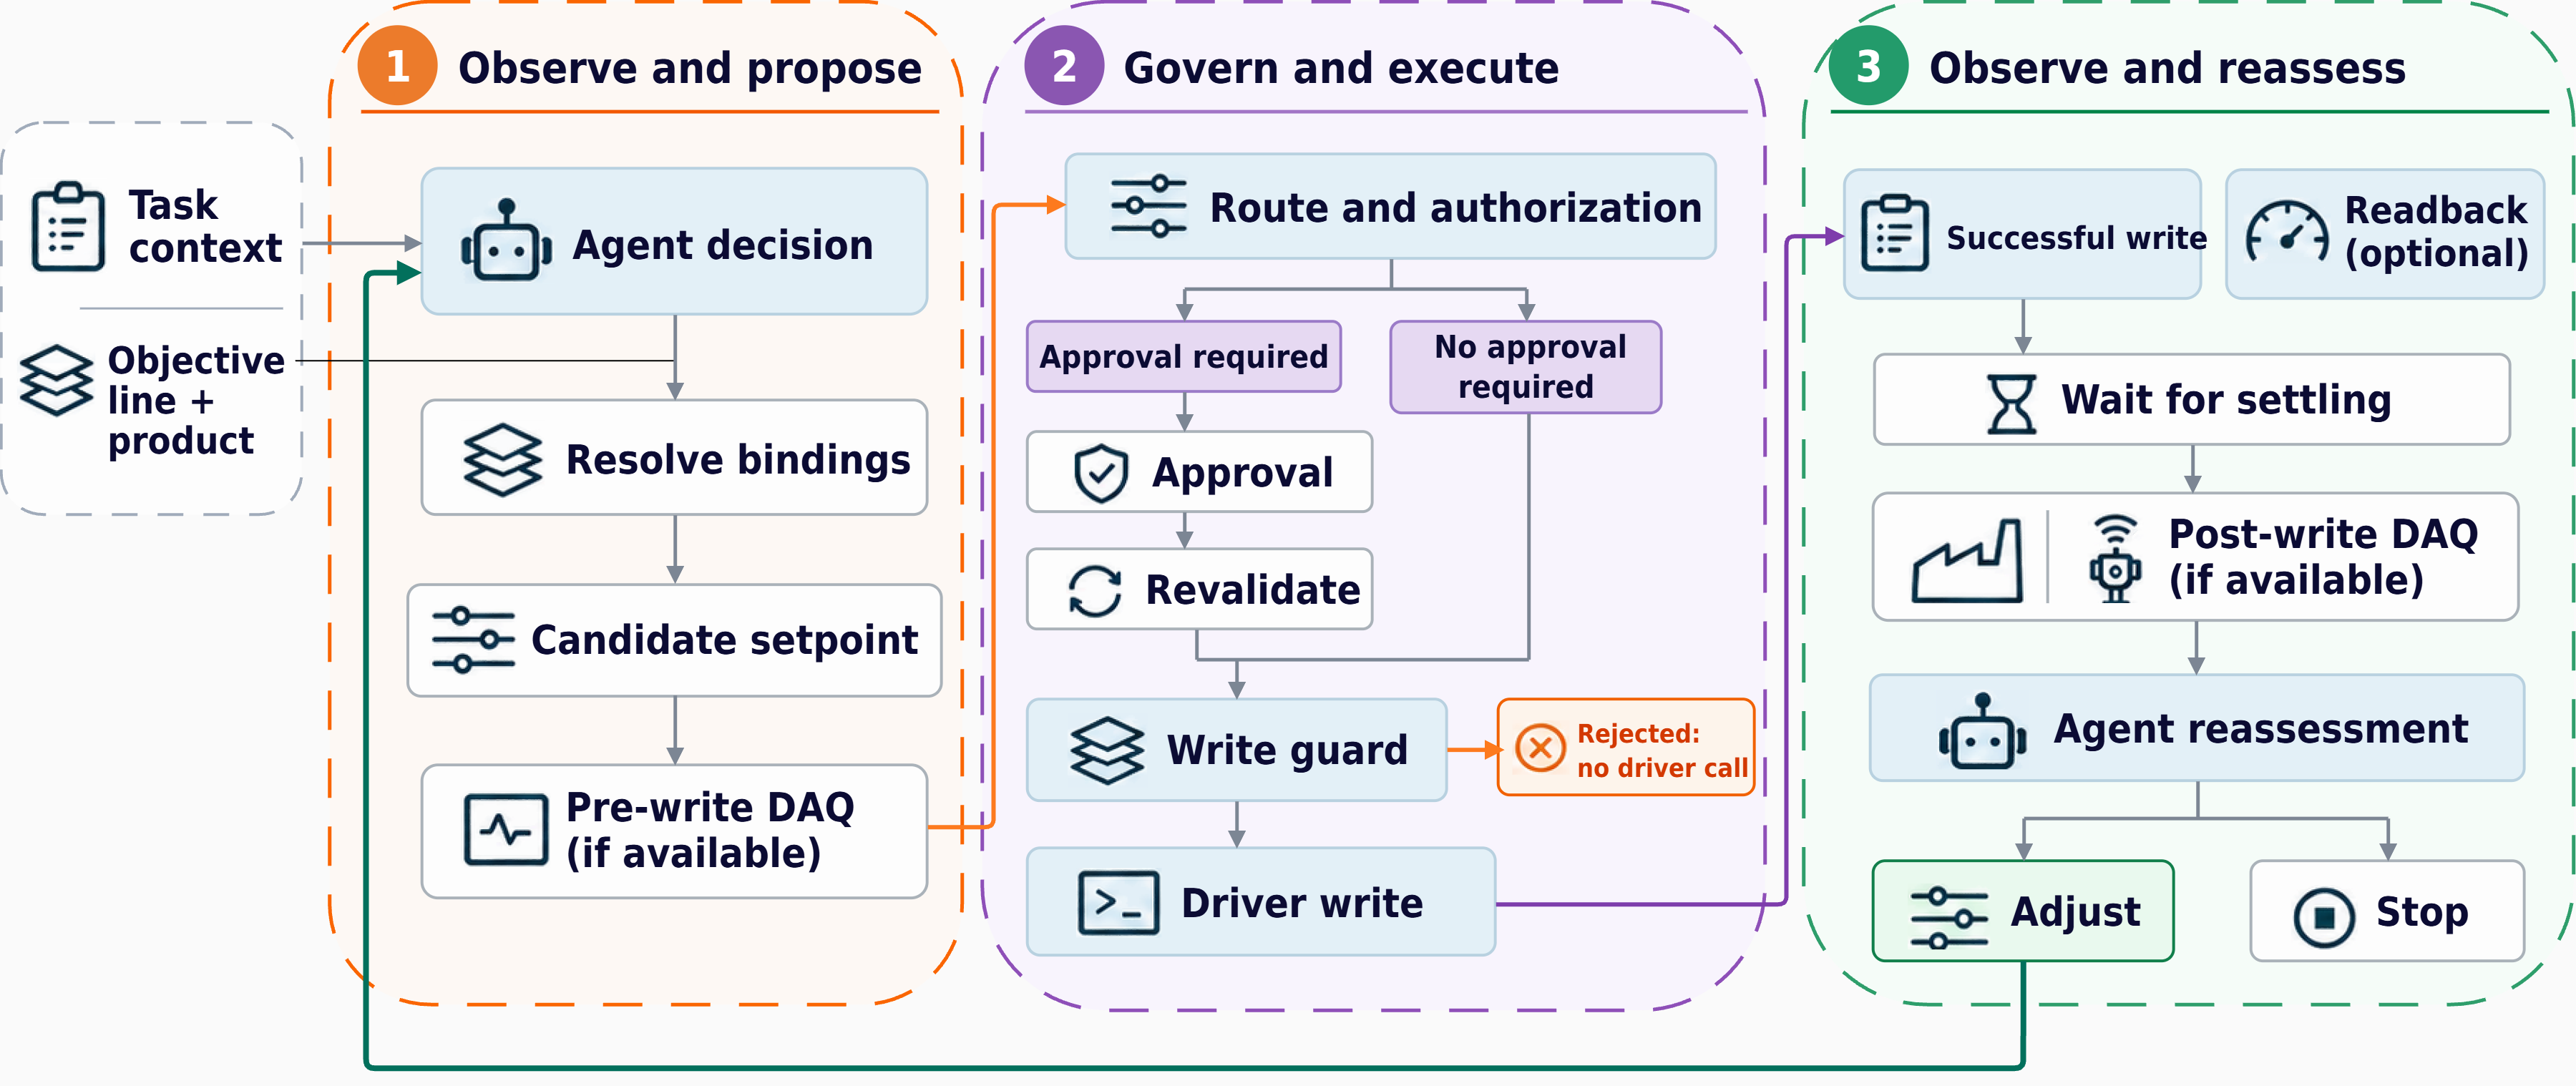
\includegraphics[width=\textwidth]{resources/fig3.png}
\caption{Agent-coordinated task workflow. The agent uses available observations to propose a setpoint. The runtime checks admission before driver dispatch and returns the command outcome, optional readback, and later DAQ observations for reassessment. The diagram shows the workflow design. Fig.~\ref{fig:hitl} details the conditional approval path.}
\label{fig:agent-loop}
\end{figure*}

A task supplies an objective and production context. The agent can acquire configured observations, compare them with the objective, and submit a typed adjustment. The workflow in Fig.~\ref{fig:agent-loop} returns operation results to the agent for the next decision. The caller can identify the control node and DAQ target explicitly. The operation uses their respective bindings when the caller omits them.

In goal mode, a lead agent can decompose the objective and assign worker subtasks. A worker can call \texttt{optimization\_explore} to request a single-node adjustment and collect process measurements around it.

In the evaluated version, the operation resolves the profile and control binding and uses the stored setpoint as $u_0$. Given a direction $s\in\{-1,+1\}$ and step $\Delta u$, it forms
\begin{equation}
 u^{*}=\operatorname{clip}\!\left(u_0+s\Delta u,\,u_{\min},\,u_{\max}\right).
 \label{eq:optimization-candidate}
\end{equation}
The operation defaults to increasing the value when no direction is supplied. In Eq.~(\ref{eq:optimization-candidate}), it clips the candidate to the configured tuning bounds or, if absent, the node bounds. It selects the step from the first available source among the explicit argument, binding, and scene limit. The default is one twentieth of the node range.

Before submitting the candidate, the operation checks that the DAQ target is visible to the caller and attempts a pre-write read. Identifiability and model--ontology checks were added after the experiments.

A valid candidate enters the governed write path in Algorithm~1. A pre-dispatch denial stops the request. If an error occurs during driver execution, the caller must reconcile the device state before retrying.

After a successful write, the operation waits 10--300~s (45~s by default) and attempts a second DAQ read. The earlier implementation uses trailing 45-s windows. A later version uses windows anchored at the request start, so the second window can include samples taken during approval before dispatch.

The exploration record stores the target, step, available DAQ means, and write status. The command record retains the outcome and available readback. The agent receives a summary and can use it on a later turn to choose another step or stop.


